\chapter{Customizing information structure}
\label{chapter11}
\setcounter{enums}{0}


The \lingo \isi{Grammar Matrix} is an open-source starter kit for the
rapid development of HPSG/MRS-based grammars
(\citealt{bender:etal:10}).  The main idea behind the system is that
the common architecture simplifies exchange of analyses among groups
of developers, and a common semantic representation speeds up
implementation of multilingual processing systems such as machine
translation.



Roughly speaking, this system is made up of two components.  The first
one is a core grammar written in \texttt{matrix.tdl}. This contains
types and constraints that are useful for modeling phenomena in all
human languages The typed feature structure of \tdl{sign} defined in
\texttt{matrix.tdl} is represented in \figref{avm:sign-matrix}, to
which the current work adds several more attributes.

\begin{figure}
% \myexe{\enumsentence{
\caption{Typed feature structure of \tdl{sign} defined in
\texttt{matrix.tdl}}
\label{avm:sign-matrix}
%     \evnup{{
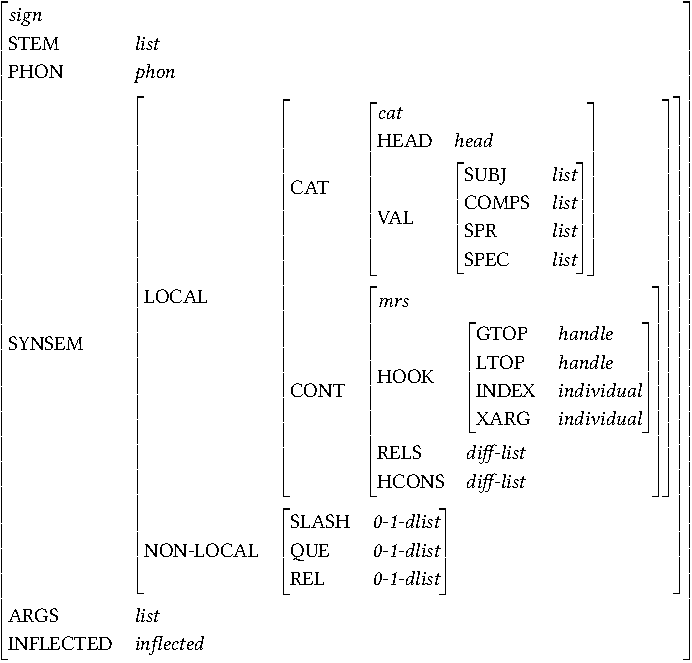
\includegraphics[width=.9\textwidth]{pdf/sign-matrix.pdf}
\end{figure}

% }}}}


\noindent The second one includes linguistic libraries for widespread,
but non-universal language phenomena
\citep{bender:flickinger:05,drellishak:09}.  The libraries work with a
customization system
(\myurl{http://www.delph-in.net/matrix/customize}).
Figure~\ref{fig:schema}, reproduced from \citet{bender:etal:10}, shows
how the \lingo \isi{Grammar Matrix} customization system operates on
the basis of user input.



\begin{figure} 
\begin{center} 
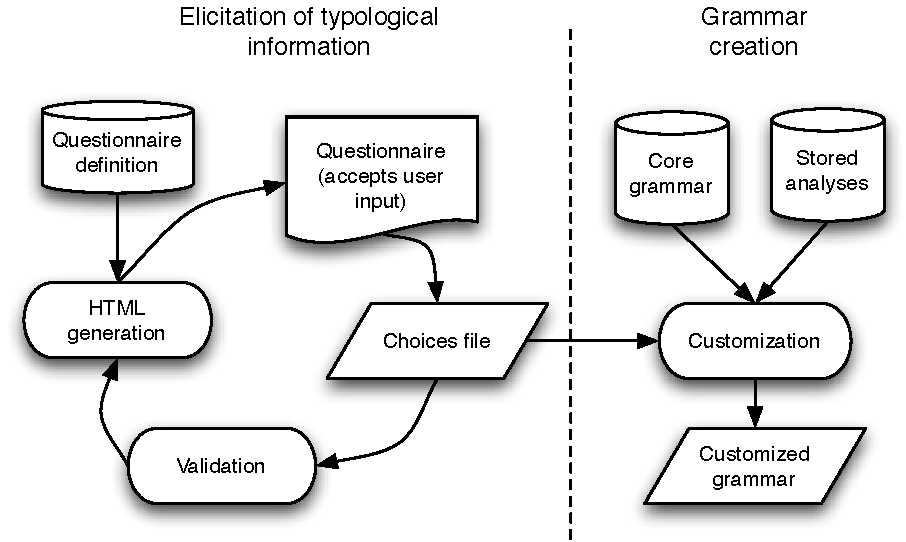
\includegraphics[width=.9\textwidth]{pdf/schema.pdf}
\caption{The \lingo Grammar Matrix customization system}
\label{fig:schema}
\end{center}
\end{figure}




\largerpage
Grammar customization with the \lingo \isi{Grammar Matrix} is provided
via a web-based questionnaire which has subpages for a series of
language phenomena.  The screenshot of the current version's main page
is shown in Figure~\ref{screenshot:main}.  For each phenomenon, the
questionnaire gives a basic explanation and questions designed to help
the user describe an analysis of the phenomenon.  After the
questionnaire has been answered, the user can press a button to
customize a grammar.  This button invokes the customization script,
which takes the user's answers stored in a \texttt{choices} file, and
first validates them for consistency, then articulates grammar
fragments into a complete grammar for the user's
language.\is{HPSG}\is{MRS} The output is an HPSG/MRS-based grammar
built automatically on the basis of specifications the user has
given. If the automatic construction is successful, a compressed file
(zip or tar.gz) is made available for download. The downloadable file
includes all required components for HPSG/MRS-based \isi{grammar
  engineering} within the \isi{DELPH-IN} formalism, so once
decompressed, the user can try out the grammar with processors such as
\isi{\lkb}~(\citealt{copestake:02}),
\isi{\pet}~(\citealt{callmeier:00}),
\isi{\agree}~(\citealt{slayden:12}),
\isi{\ace}~(\myurl{http://sweaglesw.org/linguistics/ace}), and other
\isi{DELPH-IN} software such as \isi{\itsdb}~(\citealt{oepen:01}).


\begin{figure}
\begin{center} 
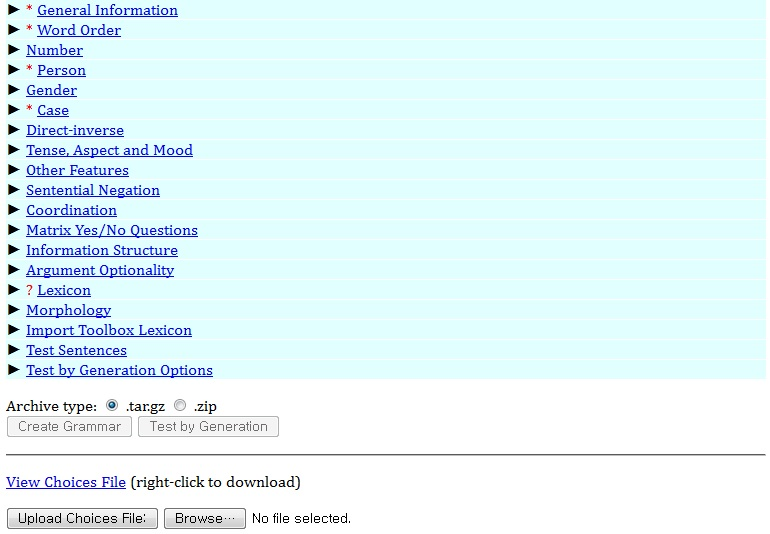
\includegraphics[width=.9\textwidth]{screenshot/ss1.jpg}
\caption{Screenshot of the questionnaire (main page)}
\label{screenshot:main}
\end{center}
\end{figure}



The grammatical categories covered in the current version are listed
in \myref{def:questionaries:1}.  The pages sometimes work
independently, and sometimes co-operate with choices given in other
subpages.  For example, users can add some additional features when
there is a need (e.g.\ animacy) on the ``Other Features'' page, which
will then appear as an option of syntactic or semantic features in
other subpages such as ``Lexicon'' and ``Morphology''.  To take
another example, the ``Sentential Negation'' page elicits information
about morphosyntactic strategies of negation in the user's language,
and specific forms of negation operators can be inserted in
``Lexicon'' and/or ``Morphology'' \citep{crowgey:12}. The
``Information Structure'' page works in a similar way.

\myexe{\enumsentence{\toplabel{def:questionaries:1}
\begin{tabular}[t]{ll}
a. & {Word Order \citep{fokkens:10}} \\ 
b. & {Number \citep{drellishak:09}} \\ 
c. & {Person \citep{drellishak:09}} \\ 
d. & {Gender \citep{drellishak:09}} \\ 
e. & {Case \citep{drellishak:09}} \\ 
f. & {Direct-inverse \citep{drellishak:09}} \\ 
g. & {Tense, Aspect and Mood \citep{poulson:11}} \\ 
h. & {Other Features \citep{drellishak:09,poulson:11}} \\ 
i. & {Sentential Negation \citep{crowgey:12}} \\ 
j. & {Coordination \citep{drellishak:bender:05}} \\ 
k. & {Matrix Yes/No Questions \citep{bender:flickinger:05}} \\ 
l. & {Information Structure (the present study)} \\ 
m. & {Argument Optionality \citep{saleem:10,saleem:bender:10}} \\ 
n. & {Lexicon \citep{drellishak:09}} \\ 
o. & {Morphology \citep{goodman:13}} \\ 
\end{tabular}}}



Four more pages not directly related to grammar creation but necessary
for ease of development are presented in \myref{def:questionaries:2}.
In the ``General Information'' page, users input supplementary
information, such as the ISO 639-3 code of the language, delimiters in
the languages, etc. The ``Import Toolbox Lexicon'' page provides an
interface to the Field Linguist's Toolbox, which is provided by SIL
(Summer Institute of Linguistics, \myurl{http://www.sil.org}).  Users
can input test sentences in the ``Test Sentences'' page, which are
included with the customized grammar for basic evaluation of the
grammar's parsing coverage. The last one provides several options for
fine-tuning the results of ``Test by Generation''.  The users can
check out the feasibility of their choices on the questionnaire
beforehand by using ``Test by Generation'', which performs the
customization in the background and displays sentences realized using
the grammar for generation with predefined semantic templates. The
users can then refine their choices based on the quality of the
results.


\myexe{\enumsentence{\toplabel{def:questionaries:2}
\begin{tabular}[t]{ll}
a. & General Information \\
b. & Import Toolbox Lexicon \\
c. & Test Sentences \\
d. & Test by Generation Options \\
\end{tabular}}}





The grammars created by the \lingo Grammar Matrix customization system
are rule-based, scalable to broad-coverage, and cross-linguistically
comparable.  The starter grammars make two contributions to
\isi{grammar engineering}. First, the starter-grammar is useful to
those who have an interest in testing linguistic hypotheses within the
context of a small implemented grammar \citep{bender:etal:11b}.
Second, starter grammars serve as a departure point to those who want
to construct broad-coverage implemented grammars, and sometimes
presents directions for improvement to an existing grammar. Thus far,
the \lingo \isi{Grammar Matrix} has been used to construct new
HPSG/MRS-based grammars (e.g.\ \isi{BURGER}, BUlgarian Resource
Grammar -- Efficient and Realistic, \citealt{osenova:11}),\il{Bulgarian}
and to improve existing grammars (e.g.\ \isi{KRG}2, \ili{Korean}
Resource Grammar \textit{ver}. 2, \citealt{song:etal:10}).




\section{Type description language}
\label{2:sec:tdl}

The grammatical fragments the current work creates are written in
\isi{TDL}.  To facilitate an understanding of the syntax, this
subsection provides a summary of \isi{TDL}.



\isi{TDL} describes feature structures within constraint-based
grammars.\footnote{\myurl{http://moin.delph-in.net/DelphinTutorial/Formalisms}}
TDL has been partially simplified and partially extended in the
reference formalism of \isi{DELPH-IN}. Thus, all processors in the
\isi{DELPH-IN} collection: \isi{\lkb}, \isi{\pet}, \isi{\ace}, and
\isi{\agree}, are fully compatible with TDL. The syntax of TDL in the
\isi{DELPH-IN} formalism has three components: (i) multiple type
inheritance, (ii) attribute-value constraints, and (iii)
coreference. For example, \myref{tdl:sample} indicates that the
current type inherits from two supertypes and that the value of an
attribute SYNSEM{$\mid$}HEAD should be consistent with the value of
the head daughter's SYNSEM{$\mid$}HEAD.

\myexe{\enumsentence{\label{tdl:sample}
\evnup{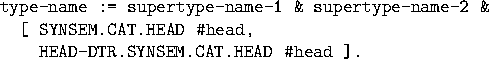
\includegraphics{pdf/tdl-sample.pdf}}}}


One of the frequently used data structures in \isi{TDL} is list. For
instance, a list \ensuremath{<}a,b,c\ensuremath{>} can be represented
as follows.

\myexe{\enumsentence{\label{tdl:list}
\evnup{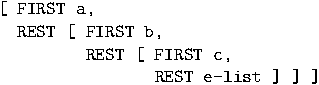
\includegraphics{pdf/tdl-list.pdf}}}}


\noindent Lists sometimes need to work more flexibly to allow
concatenation, append, removal, etc.  For these operations, the
\isi{DELPH-IN} formalism utilizes difference lists (\tdl{diff-list}).
This structure maintains a pointer to the last element of the list.
Analogously to \myref{tdl:list}, a difference list \ensuremath{<}!
a,b,c !\ensuremath{>} can be represented as in \myref{tdl:diff-list}.

\myexe{\enumsentence{\label{tdl:diff-list}
\evnup{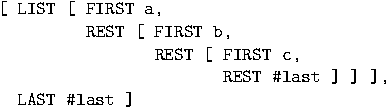
\includegraphics{pdf/tdl-diff-list.pdf}}}}





\section{The questionnaire}
\label{11:sec:questionnaire}

The first task of implementing the customization system's information
structure library centers around adding an HTML-based page to the
web-based questionnaire.  The ``Information Structure'' page is
comprised of four sections, namely ``Focus'', ``Topic'', ``Contrastive
Focus'', and ``Contrastive Topic''.\is{lexical markers}\is{contrastive
  topic}\is{contrastive focus} Each section, except the last one,
consists of two subparts:\is{syntactic positioning} one for syntactic
positioning and the other for lexical marking(s).



\subsection{Focus}
\label{11:ssec:questionnaire-focus}


First, in the ``Focus'' section, users can specify the canonical
position of \isi{focus} in the user's language. A screenshot is shown in
Figure~\ref{screenshot:focus}.  According to the cross-linguistic
survey given in Chapter~\ref{chapter4}
\mypage{4:ssec:focus-position}, there are four options:
\isi{clause-initial}, \isi{clause-final}, \isi{preverbal}, and
\isi{postverbal}.  A sentence in the neutral word order is a default
form in the language, which can be interpreted as conveying a range of
information structure values. For example, if SVO is the default order
in a language, we cannot look at postverbal or clause-final [O] as
being marked for
\tdl{focus}.\is{\textit{info-str}}\is{clause-final}\is{focus}



\begin{figure} 
\begin{center} 
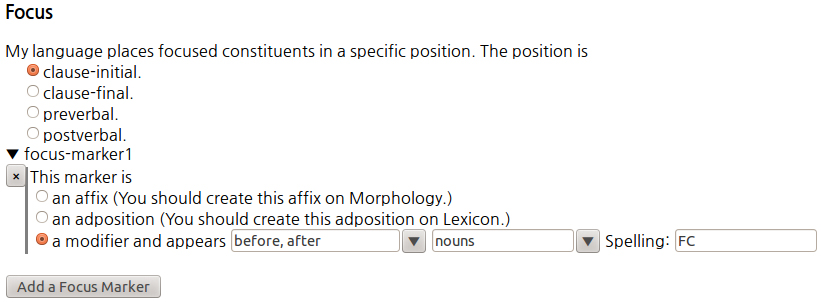
\includegraphics[width=.9\textwidth]{screenshot/focus.jpg}
\caption{Screenshot of editing focus position/markers in the questionnaire}
\label{screenshot:focus}
\end{center}
\end{figure}

\newpage 
Users can add one or more \isi{focus} markers.\is{adposition} The type
of a focus marker is either an affix, an adposition, or a modifier as
surveyed in Section \ref{4:sec:lexical}
\mypage{4:sec:lexical}. Affixes are treated in the morphological
paradigm (i.e.\ \texttt{irules.tdl}), while the other two are treated
like a word (i.e.\ \texttt{lexicon.tdl}). The distinction between the
last two is also discussed in Section \ref{4:sec:lexical}:\is{lexical markers}
If a language employs case-marking adpositions and a lexical marker to
express focus and/or \isi{topic} is in complementary distribution with
the case-marking adpositions, the marker is categorized as an
adposition in principle. Otherwise, the marker is treated as just a
modifier.\footnote{Nonetheless, the users of the \lingo Grammar Matrix
  system may have the flexibility to describe what the users see in
  their language following the meta-modeling idea of \citet{poulson:11}.}
Specific forms for information-structure marking affixes and
adpositions are not specified in the ``Information Structure'' page,
and instead they should be defined in the ``Morphology'' and
``Lexicon'' pages, respectively. If users select that their language
has an affix or an adposition of expressing \isi{focus} in the
``Information Structure'' page, but an affix or an adposition that
involves \tdl{focus} or super/sub-types of \tdl{focus} as a value of
``information-structural meaning'' is not added in the ``Morphology''
or ``Lexicon'' pages, a validation error is produced. The spelling of
information-structure marking modifier(s) is directly specified on the
``Information Structure'' page, because there is no room for such an
expression (e.g.\ particles, clitics, etc.) in ``Morphology'' and
``Lexicon''.  Users can specify more constraints on
information-structure marking modifier(s), such as before and/or after
nouns and/or verbs.





For instance, Figure~\ref{screenshot:focus} is illustrative of users'
choices on ``Focus''. As mentioned earlier in
Section \ref{4:ssec:categorical} \mypage{4:ssec:categorical}, one lexical
marker may be used to signal \isi{focus} to both nominal and verbal
items.\is{lexical markers} One lexical marker may occur sometimes before focused
constituents and sometimes after them. Thus, the users can take
multiple options for the constraints, as presented as [before, after]
in Figure~\ref{screenshot:focus}.



\subsection{Topic}
\label{11:ssec:questionnaire-topic}


Second, the ``Topic'' section has two choices for constraints. As for
the constraint on positioning, an option for the topic-first
restriction is provided for the languages in which \isi{topic} always
occupies the sentence-initial position. Next, one or more topic
markers can be added, which operate in the same way as the ``Add a
Focus Marker'' button discussed above.  As shown in
Section \ref{3:sssec:verbal-topics} \mypage{3:sssec:verbal-topics}, verbal
items can be topicalized in some languages
(e.g.\ \ili{Paumar{\'{\i}}}, \citealt{chapman:81}).  Thus, [verbs] in
Figure~\ref{screenshot:topic} is selected for illustrating the
language-specific constraint.

\begin{figure}[!t]
\begin{center} 
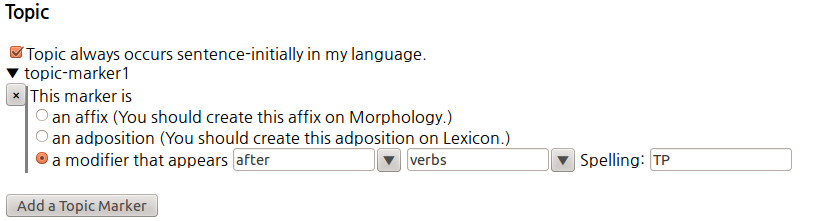
\includegraphics[width=.9\textwidth]{screenshot/topic.jpg}
\caption{Screenshot of editing topic position/markers in the questionnaire}
\label{screenshot:topic}
\end{center}
\end{figure}





\subsection{Contrastive focus}
\label{11:ssec:questionnaire-cf}

Third, \isi{contrastive focus} may or may not be marked differently
from \is{non-contrastive focus} non-con\-tras\-tive focus, which is language-specific. If the
first checkbox in Figure~\ref{screenshot:cf} (just under the title
``Contrastive Focus'') is not selected, there can be two types of
foci: one is \tdl{semantic-focus} for non-contrastive focus, and the
other is \tdl{contrast-focus} for contrastive focus. In the latter
case, users have to choose a specific position for contrastive focus,
such as \isi{clause-initial}, \isi{clause-final}, \isi{preverbal}, or
\isi{postverbal}. If users do not choose one of them, the validation
script gives an error message.  Contrastive focus markers are added
using the same tools and selectors as other markers.


\begin{figure}[!t]
\begin{center} 
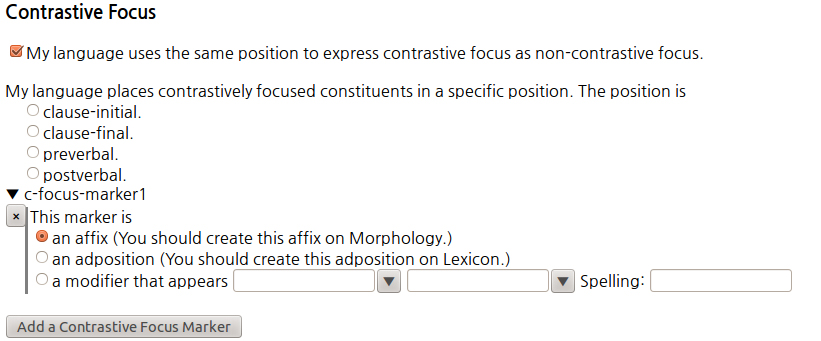
\includegraphics[width=.9\textwidth]{screenshot/cf.jpg}
\caption{Screenshot of editing contrastive focus position/markers in the questionnaire}
\label{screenshot:cf}
\end{center}
\end{figure}


\subsection{Contrastive topic}
\label{11:ssec:questionnaire-ct}

Finally, there is an option for ``Contrastive Topic''.\is{contrastive
  topic} According to the cross-lin\-guis\-tic survey the present study
has conducted, there seems to be no language in which contrastive
topics have a constraint on positioning, and this is also supported by
several previous analyses
\citep{choi:99,erteschik:07,bianchi:frascarelli:10}. Accordingly,
there is no checkbox for adding a position constraint. On the other
hand, some languages employ a \isi{contrastive topic} marker
(e.g.\ \textit{th{\`i}} in Vietnamese, \citealt{nguyen:06}). These can
also be specified using the button ``Add a Contrastive Topic Marker''.

\begin{figure}[!t]
\begin{center} 
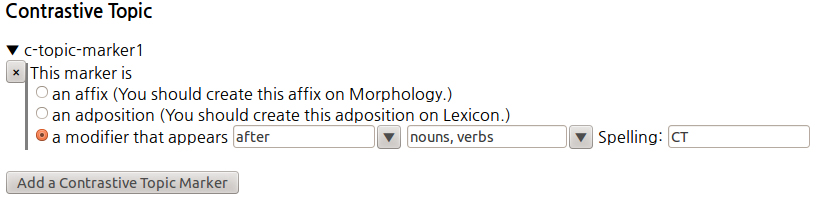
\includegraphics[width=.9\textwidth]{screenshot/ct.jpg}
\caption{Screenshot of editing contrastive topic markers in the questionnaire}
\label{screenshot:ct}
\end{center}
\end{figure}



\section{The Matrix core}
\label{11:sec:matrix}




The next task was to incorporate the analysis based on ICONS
(Individual CONStraints)\is{Individual CONStraints} into the Matrix
core. The core \isi{TDL} fragments written in \texttt{matrix.tdl}
define universally useful types in widespread linguistic phenomena.
Notably, integrating \isi{ICONS} into the grammar requires editing
lots of previously implemented types as well as adding several new
types. This is because I am concerned not merely with the
representations (implemented via changes to MRS and the addition of
the actual type for ICONS),\is{MRS} but also with their composition at
the syntactic level.  Thus, I had to revise many lexical rules and
types inherited by almost all phrase structure rules and lexical
rules.  The details are as follows.




\subsection{Fundamentals}
\label{11:ssec:fundamentals}


First of all, three type hierarchies presented in
Chapter~\ref{chapter9}, such as \tdl{info-str}, \tdl{mkg}, and
\tdl{sform},\is{sentential forms}\is{\textit{sform}} were
added.\is{MKG}\is{ICONS-KEY}\is{\textit{info-str}}\is{\textit{mkg}}\is{\textit{sform}}
Then, [MKG \tdl{mkg}] was added into CAT, and CONT values were also
edited as containing ICONS-related features, such as [ICONS-KEY
  \tdl{icons}] and [CLAUSE-KEY \tdl{event}] under \tdl{hook}, and
[ICONS \tdl{diff-list}] under \tdl{mrs}. The \isi{TDL} statements for
representing \tdl{info-str} is presented in \myref{tdl:info-str}
(cf.\ Figure~\ref{fig:info-str}).\is{CLAUSE-KEY}\is{ICONS}\is{\textit{info-str}}


\myexe{\enumsentence{\label{tdl:info-str}
\evnup{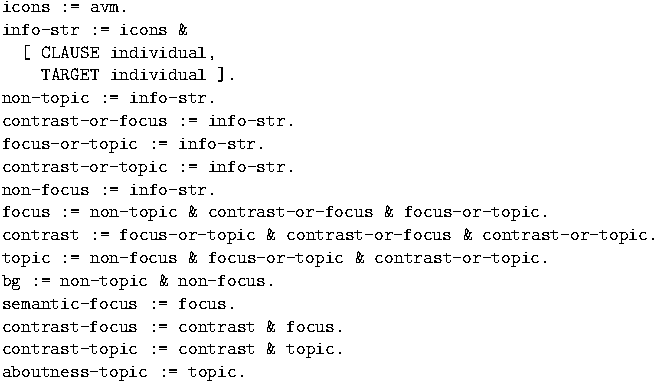
\includegraphics{pdf/tdl-info-str.pdf}}}}




\noindent \isi{ICONS} were added into the basic lexical and phrasal
types in \texttt{matrix.tdl} (e.g.\ \tdl{unary-phrase},
\tdl{binary-phrase}, \tdl{ternary-phrase}, etc.). Next, I specifically
inserted \mbox{[C-CONT{$\mid$}ICONS \ensuremath{<}!  !\ensuremath{>}]}
into phrase structure rules and lexical rules: when a lexical or
phrasal type has nothing to do with information structure,
C-CONT{$\mid$}ICONS is specified as an empty list.




\subsection{Lexical types}
\label{11:ssec:lt}



Regarding lexical types, the set of types used for marking \tdl{icons}
within a lexical item, such as \tdl{no-icons-lex-item},
\tdl{basic-icons-lex-item}, \tdl{one-icons-lex-item}, and
\tdl{two-icons-lex-item} (Section \ref{10:sec:lexical}), were written as
\isi{TDL} statements. Lexical types for constraining ARG-ST
(ARGument-STructure) inherit from one of them and impose some
additional constraints on CLAUSE-KEY.  For example,
\tdl{intransitive-lex-item}, which places a constraint on ARG-ST of
intransitive verbs, is defined as in
(\ref{tdl-basic-icons-lex-item:b}). Note that this type inherits from
\tdl{basic-icons-lex-item} that has an empty \isi{ICONS} list as shown
in (\ref{tdl-basic-icons-lex-item:a}).  There is a coreference tag
\texttt{\#clause} in (\ref{tdl-basic-icons-lex-item:b}), which
indicates that every argument shares the value of CLAUSE-KEY with the
semantic head within a single clause.


\myexe{\enumsentence{\label{tdl-basic-icons-lex-item:a}
\evnup{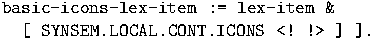
\includegraphics{pdf/tdl-basic-icons-lex-item.pdf}}}}

\myexe{\enumsentence{\label{tdl-basic-icons-lex-item:b}
\evnup{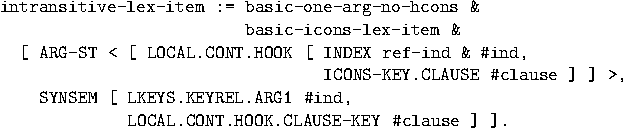
\includegraphics{pdf/tdl-intransitive-lex-item.pdf}}}}




\noindent Some lexical types inherently include an \tdl{info-str}
value.\is{\textit{info-str}} In this case, lexical types for ARG-ST
impose a constraint on the element of \tdl{info-str}.  For instance,
the type \tdl{clausal-second-arg-trans-lex-item}, which is responsible
for the AGT-ST of verb classes which take a clausal complement
(e.g.\ \textit{think}, \textit{ask}), is defined as shown in
(\ref{tdl-one-icons-lex-item:b}) (see Section \ref{10:ssec:embedded}).  Note
that the INDEX of the second argument (i.e.\ a clausal complement) and
the TARGET of the element in the \isi{ICONS} list are co-indexed
(\texttt{\#target}).



\myexe{\enumsentence{\label{tdl-one-icons-lex-item:a}
\evnup{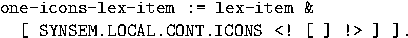
\includegraphics{pdf/tdl-one-icons-lex-item.pdf}}}}


\myexe{\enumsentence{\label{tdl-one-icons-lex-item:b}
\evnup{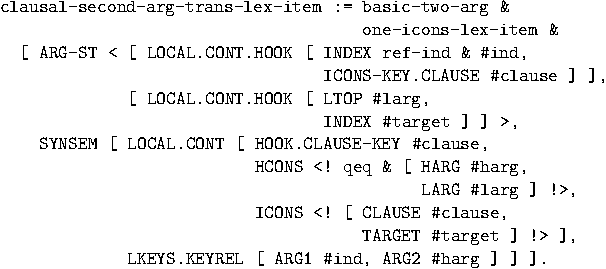
\includegraphics{pdf/tdl-clausal-second-arg-trans-lex-item.pdf}}}}






\subsection{Lexical rules}
\label{11:ssec:lr}

There are two types of lexical rules. One introduces an element of
\tdl{info-str} into C-CONT{$\mid$}ICONS,\is{\textit{info-str}} and the
other does not.  In order to support these types, I needed to change
\tdl{no-ccont-rule} to include \mbox{[C-CONT{$\mid$}ICONS
    \ensuremath{<}!  !\ensuremath{>}]} and to add a type that allows
for a non-empty \isi{ICONS} list. This type is called
\tdl{no-rels-hcons-rule}, and constrains RELS and HCONS to be empty
while leaving ICONS underspecified.\is{underspecification} These rules
are also used for phrase structure rules as well.


\subsection{Phrase structure rules}
\label{11:ssec:phr}


First, \tdl{basic-head-subj-phrase}, \tdl{basic-head-comp-phrase},
\tdl{basic-head-spec-phrase} as well as \tdl{basic-bare-np-phrase} inherit
from \tdl{no-ccont-rule}. Therefore, they have an empty \isi{ICONS}
list.  Second, I edited two phrase structure rules for argument
optionality,\is{argument optionality} namely
\tdl{basic-head-opt-subj-phrase} and
\tdl{basic-head-opt-comp-phrase}.\is{argument optionality} They
introduce an \isi{ICONS} element that indicates the value of
information structure the dropped argument has (i.e.\ \tdl{non-focus})
into C-CONT{$\mid$}ICONS. This constraint is in line with my analysis
presented in Section \ref{10:sec:arg-opt} \mypage{avm:opt}.  Third, I modified
\tdl{basic-head-mod-phrase-simple} (a subtype of
\tdl{head-mod-phrase}) in accordance with the AVM presented in
Section \ref{10:sec:monoclausal} \mypage{avm:head-mod-phrase}: now it has an
empty list in C-CONT{$\mid$}ICONS, and the CLAUSE-KEY of modifiers
(NON-HEAD-DTR) and that of their modificands are co-indexed with each
other.\is{CLAUSE-KEY} Finally, \tdl{head-filler-phrase} does not
include \mbox{[C-CONT{$\mid$}ICONS \ensuremath{<}!
    !\ensuremath{>}]}. This is because its subtypes sometimes
constructionally introduce an element of
\tdl{info-str}.\is{\textit{info-str}}\is{clause-initial}\is{clause-final}
For example, clause-initial and clause-final \isi{focus} in languages
with a \isi{fixed word order} are instances of
\tdl{head-filler-phrase}, and introduce an element into
C-CONT{$\mid$}ICONS.  The remaining part of a sentence which has a
syntactic gap is constrained by \tdl{basic-head-subj-nmc-phrase} or
\tdl{basic-head-comp-nmc-phrase}, in which \tdl{nmc} stands for
non-matrix-clause.  These rules work for \tdl{head-subj-phrase} and
\tdl{head-comp-phrase} that cannot be root nodes by themselves
(i.e. specified as \mbox{[MC --]}). These phrases are supposed to be
combined only with a \tdl{filler-phrase}.  There is one more phrase
structure rule related to \tdl{filler-phrase}:
\tdl{nc-filler-phrase}. This rule handles a non-canonical
\tdl{filler-phrase}; for example, detached constituents in right
dislocation.





\section{Customized grammar creation}
\label{11:sec:creation}

The third task is to implement the Python code to customize the users'
choices. The code first validates the content in the \texttt{choices}
file to check for inconsistencies and missing inputs. If no error
occurs, then the code converts the content in the \texttt{choices}
file into \isi{TDL} statements.


\myexe{\enumsentence{\toplabel{tdl:sample-choices}
\evnup{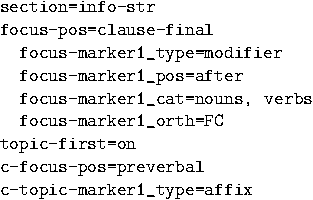
\includegraphics{pdf/tdl-sample-choices.pdf}}}}


The users' answers about information structure are stored in a
\texttt{choices} file as shown in \myref{tdl:sample-choices}. The
choices shown in \myref{tdl:sample-choices} specify that the language
places a focused constituent in the clause-final
position,\is{clause-final} and employs a focus marker, which is a
single word spelled as `\texttt{FC}' appearing after nouns or
verbs. The language is a topic-first language as indicated by
`\texttt{topic-first=on}'. The language uses a different place for
signaling contrastive \isi{focus}. In this case, it is the
\isi{preverbal} position. Finally, the language has an affix
responsible for conveying a meaning of \isi{contrastive topic}, which
should be defined in the ``Morphology'' page.  Those choices are
transmitted into the customization script for information structure.




\subsection{Lexical markers}
\label{11:ssec:lex}

There are three types of lexical markers: (i) affixes, (ii)
adpositions,\is{adposition} and (iii) modifiers. Among them, the
first one and the second one are specified in the ``Morphology'' and
``Lexicon'' pages respectively.  They are handled by existing
customization code, which works seamlessly with the
information-structure related features and values enabled by the
information structure library.  I edited two existing customization
libraries for the first two options and the script for information
structure (i.e.\ \texttt{information{\_}structure.py}) creates only
the last type of marker.






(i) Affixes are customized by \texttt{morphotactics.py}.  If a lexical
rule imposes a constraint on information structure meaning, the
lexical rule inherits from \tdl{no-rels-hcons-rule} (explained before
in (Section \ref{11:ssec:lr}) and introduces an element of \tdl{info-str} into
C-CONT{$\mid$}ICONS.\is{\textit{info-str}} Otherwise, it inherits just
from \tdl{add-only-no-ccont-rule} (or other lexical rules with an
empty C-CONT{$\mid$}ICONS). For instance, the TDL statements
presented in \myref{tdl:affix} are responsible for a focus-marking
suffix, and introduces a value of \tdl{info-str} into ICONS. Note the
two coreference tags in \tdl{add-icons-rule}, namely \#icons and
\#target.


\myexe{\enumsentence{\toplabel{tdl:affix}
\evnup{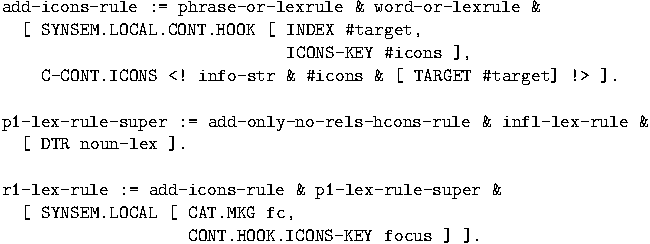
\includegraphics{pdf/tdl-affix.pdf}}}}


(ii) Adpositions are dealt with by
\texttt{lexical\_items.py}.\is{adposition} Likewise, an \isi{ICONS} list of an adposition
is constructed depending on whether an adposition has a feature that
constrains the semantics related to information structure. An instance
is provided in \myref{tdl:adp}. In this case, the adposition lexically
includes a value of \tdl{info-str} in CONT{$\mid$}ICONS, and the
TARGET is co-indexed with the INDEX of the complement. This works in
the same manner as \ga and \wa in \ili{Japanese} as presented
previously in Section \ref{9:ssec:jpn:kor} \mypage{avm:ga:wa:jpn}.

\myexe{\enumsentence{\toplabel{tdl:adp}
\evnup{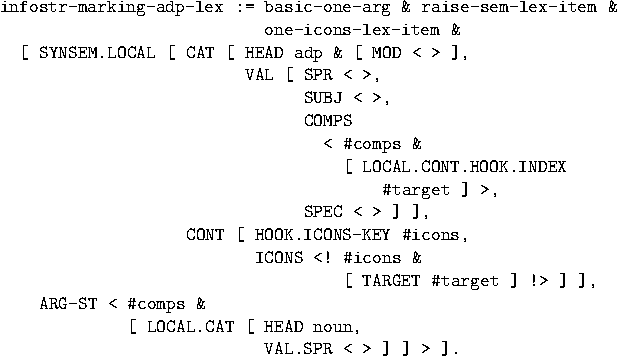
\includegraphics{pdf/tdl-adp.pdf}}}}




(iii) Finally, \texttt{information{\_}structure.py} creates TDL
statements for information-structure marking modifiers, and depending
on the specific choices, the lexical types are also elaborated. For
example, the choices in \myref{tdl:sample-choices} yield the following
TDL statements given in
(\ref{tdl:modifiers:types:a}-\ref{tdl:modifiers:types:b}). The \isi{TDL}
statements presented in
(\ref{tdl:modifiers:types:a}-\ref{tdl:modifiers:types:b}) define the
lexical type of modifiers that mark information
structure.\is{adposition} Like the information-structure marking
adpositions shown above, a value for \tdl{info-str} is lexically
included in CONT{$\mid$}ICONS, but the TARGET is co-indexed with the
INDEX of its modificand.


\myexe{\enumsentence{\label{tdl:modifiers:types:a}
\evnup{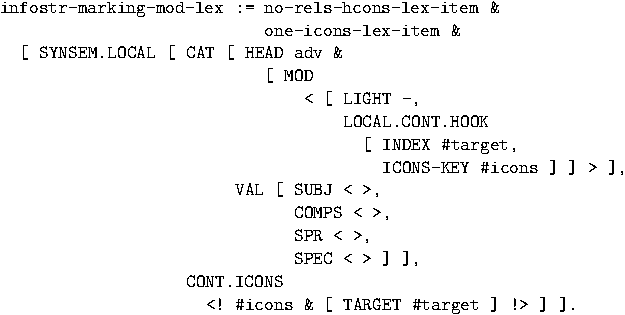
\includegraphics{pdf/tdl-infostr-marking-mod-lex.pdf}}}}

\myexe{\enumsentence{\label{tdl:modifiers:types:b}
\evnup{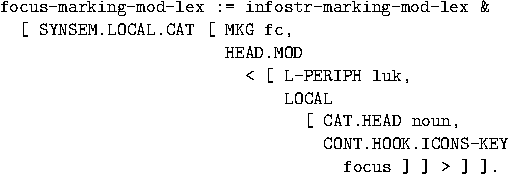
\includegraphics{pdf/tdl-focus-marking-mod-lex.pdf}}}}



\noindent Since a modifier and its modificand are combined with each
other by a phrase structure rule, the customization script
additionally creates some \isi{TDL} statements related to
\tdl{head-mod-phrase}. For example, if the language employs an
information-structure marking modifier and the modifier appears after
its modificand, \tdl{head-adj-int-phrase} (a subtype of
\tdl{basic-head-mod-phrase-simple}) and \tdl{head-adj-int} are
inserted into \texttt{mylang.tdl} and \texttt{rules.tdl},
respectively. Additionally, an entry for the information-structure
marking modifier is specified in \texttt{lexicon.tdl}.




\subsection{Syntactic positioning}
\label{11:ssec:ph}



The customization script \texttt{information\_structure.py} also
creates grammatical fragments in TDL for constraining \isi{focus} or \isi{topic}
in a specific position. As an initial step, the script merges the
users' choices into a single type. For example, if a language places
focused constituents in the clause-initial position and the language
has the topic-first restriction, clause-initial constituents
ex situ are specified as \tdl{focus-or-topic} in the
language.\is{clause-initial}



As mentioned in Section \ref{11:ssec:phr}, languages with a \isi{fixed word
  order} (e.g.\ SVO, SOV, VSO, VOS, OSV, and OVS) employ a specific
type of \tdl{head-filler-phrase} for clause-initial and clause-final
\isi{focus} and clause-initial
\isi{topic}.\is{clause-initial}\is{clause-final} In other words, the
focused and topicalized constituents fill out the syntactic gap of the
remaining part of a sentence. The remaining part of the sentence is
realized as non-main-clausal constituents
(e.g.\ \tdl{head-nmc-subj-phrase} and \tdl{head-nmc-comp-phrase}),
which (i) have a nonempty list in NON-LOCAL{$\mid$}SLASH, and flag
features indicating (ii) the phrase cannot be a main clause
(i.e.\ \mbox{[MC --]}), and (iii) the phrase is not peripheral
(i.e.\ \mbox{[L-PERIPH --, R-PERIPH
    --]}).\is{L-PERIPH}\is{R-PERIPH}\is{periphery} Such a phrasal type
with the \tdl{nmc} prefix should be combined with phrases with
\mbox{[L-PERIPH +]} or \mbox{[R-PERIPH +]} to constitute a
\tdl{infostr-filler-head-phrase}.  The assignment of an \tdl{info-str}
value is carried out by \tdl{infostr-dislocated-phrase} presented in
(\ref{tdl:filler:a}). The gap is filled in by
\tdl{infostr-filler-head-phrase} presented in
(\ref{tdl:filler:b}).\footnote{In the case of right dislocation,
  \tdl{infostr-head-filler-phrase} which inherits from
  \tdl{nc-filler-phrase} instead of \tdl{basic-head-filler-phrase} is
  used.} Since this type specifies \mbox{[L-PERIPH --]} on itself, no
further combination to the left side is allowed.






\myexe{\enumsentence{\label{tdl:filler:a}
\evnup{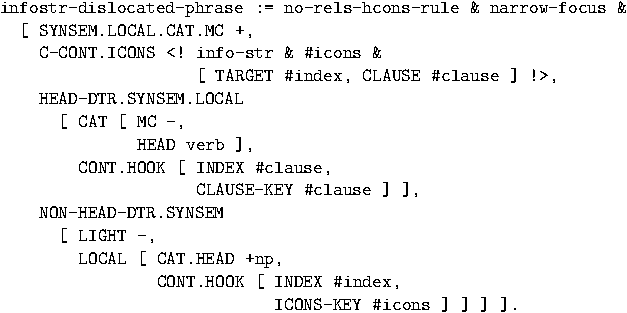
\includegraphics{pdf/tdl-infostr-dislocated-phrase.pdf}}}}


\myexe{\enumsentence{\label{tdl:filler:b}
\evnup{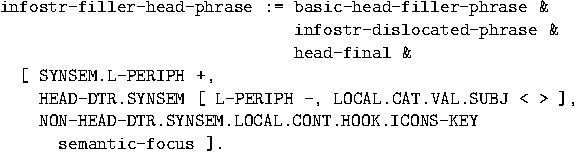
\includegraphics{pdf/tdl-infostr-filler-head-phrase.pdf}}}}






If the user's language employs a \isi{fixed word order}, \isi{preverbal} and
\isi{postverbal} \isi{focus} is constrained not by \tdl{head-filler-phrase}, but
by specific types of \tdl{head-subj-phrase} and
\tdl{head-comp-phrase}.  Since \isi{preverbal}/\isi{postverbal} foci are
immediately adjoined to the verb or the verb cluster,\footnote{See the
  Basque example presented in Section \ref{9:ssec:lightness}
  \mypage{exe:urbina:focus:ch10-1}, in which the subject is combined
  with a verb plus an auxiliary.\is{auxiliary}} 
  they do not behave as a syntactic filler.\is{lightness}
Such a specific phrasal type imposes \mbox{[LIGHT +]} on the
HEAD-DTR and \mbox{[ICONS-KEY \tdl{focus}]} (or a subtype of
\tdl{focus}) on the NON-HEAD-DTR.\is{ICONS-KEY}
What is significant here is using a
flag feature, namely INFOSTR-FLAG.  This feature indicates whether a
constituent can be used as the \isi{preverbal} and \isi{postverbal}
focus. \tdl{Narrow-focused-phrase},\is{narrow focus} presented in (\ref{tdl:nf:a}), is a
unary phrase structure rule that specifies the plus value of
INFOSTR-FLAG and introduces an element into ICONS. Only constituents
with \mbox{[INFOSTR-FLAG +]} can be narrowly focused as constrained by
\tdl{head-nf-comp-phrase-super} given in (\ref{tdl:nf:b}) (or
\tdl{head-nf-subj-phrase-super}).\is{\textit{info-str}} The specific value of \tdl{info-str}
(e.g.\ \tdl{focus}) is assigned by \tdl{nf-comp-head-phrase} (or its
siblings) presented in (\ref{tdl:nf:c}).



\myexe{\enumsentence{\label{tdl:nf:a}
\evnup{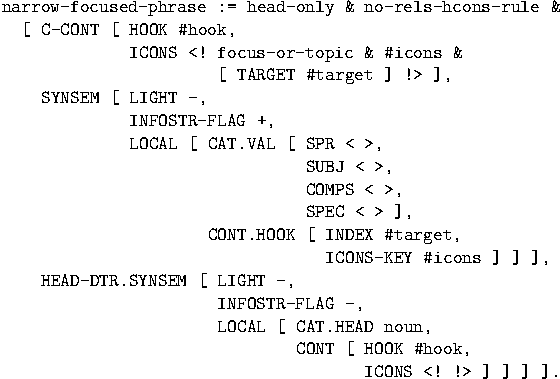
\includegraphics{pdf/tdl-narrow-focused-phrase.pdf}}}}

\myexe{\enumsentence{\label{tdl:nf:b}
\evnup{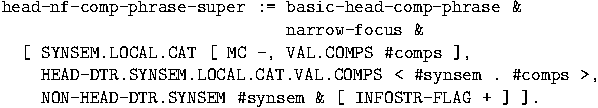
\includegraphics{pdf/tdl-nf-super.pdf}}}}

\myexe{\enumsentence{\label{tdl:nf:c}
\evnup{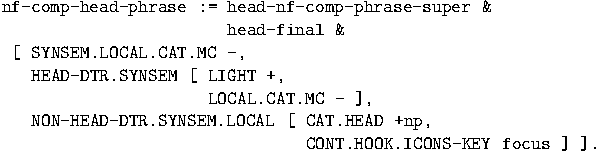
\includegraphics{pdf/tdl-nf.pdf}}}}




\noindent When these constraints are included in users' grammar, other
ordinary phrase structure rules have an additional constraint:
\mbox{[INFOSTR-FLAG +]} on themselves and their daughter(s).



If the word order is flexible (e.g.\ v-final and v-initial), no
subtype of \tdl{head-filler-phrase} is introduced. Instead,
\tdl{head-subj-phrase} and/or \tdl{head-comp-phrase} become twofold,
depending on the positioning constraint(s).  Such a twofold strategy
is the same as how scrambling in \ili{Japanese} and \ili{Korean} is
constrained with respect to information structure roles
(Section \ref{10:sec:scrambling}).\is{\textit{info-str}} In this case, the
flag feature INFOSTR-FLAG is also used, because arguments ex
situ introduce an \tdl{info-str} element into \isi{ICONS} while
arguments in situ do not. INFOSTR-FLAG serves to make a
distinction between them. That is, this strategy is almost the same as
that in languages that employ a \isi{fixed word order} and place
focused constituents in the \isi{preverbal} or \isi{postverbal}
position. The same goes for V2 languages.\is{V2 languages}  If a language employs the
V2 word order (e.g.\ \ili{Yiddish}), all information structure-marked
constituents are dealt with in the same way as in
(\ref{tdl:nf:a}-\ref{tdl:nf:c}).  Section \ref{12:sec:collage} shows how
information structure in V2 languages is customized with reference to
two particular V2 languages: \ili{Frisian} and \ili{Yiddish}.


There is still room for refinement, which should be studied in future
work.  First, the treatment of free word order languages
(e.g.\ \ili{Russian}) could be improved.  It is reported that word
ordering variation in in such languages largely depends on information
structure \citep{rodionova:01}.  Grammatical modules for constraining
positions of information structure components in free word order
languages should be designed in tandem with a study of the full range
of word order possibilities. Second, \tdl{head-filler} also predicts
the possibility of long-distance dependencies, which are not fully
tested in the present work. Whether or not using \tdl{head-filler} for
constraining information structure causes unforeseen side effects
should be thoroughly investigated in future work.








\section{Regression testing}
\label{12:sec:pseudo}


When developing a grammar library, regression testing using
\isi{testsuites} (a collection of sentences intended to demonstrate
the capabilities of the implementation, \citealt{bender:etal:07}) is crucial. 
Using a set of testsuites, regression testing
checks if a new implementation works well with all the previous
functionality in the development of software.  That is to say,
regression testing ensures that the newly adapted development is not
detrimental to the previous implementation.  I ran the regression
tests from all previous libraries in order to confirm that my library
did not break anything, and then added regression tests to document
the current library for information structure.\is{regression test}





\subsection{Testsuites}
\label{12:ssec:testsuites}


The first step is to develop pseudo languages, picking up hypothetical
types of languages that that show the full range of information
structure marking systems and to write down sentences for each pseudo
language. The testsuites represent abstract language types in the
space defined by ``Information Structure'' library.


Testsuites for pseudo languages consist of pseudo words that stand for
sentential configurations. Each pseudo word indicates its linguistic
category, similar to glosses in interlinear annotation. For example,
CN in the string stands for `Common Noun', IV for `Intransitive Verb',
TV for `Transitive Verb', and so on. The linear order of the elements
within strings simulates the word order. For instance, ``CN IV'' is an
instance of an intransitive sentence like \textit{Dogs bark.}  In the
pseudo languages that I created for testing this library, there are
several specific strings that simulate an \tdl{info-str}
role.\is{adposition} For instance, a morpheme `-FC' or a separate word
(i.e.\ an adposition and a modifier) `FC' (FoCus), can be used in
languages that employ lexical markers to yield focus meaning. For
example, ``CN-FC IN'' carries an information structure meaning similar
to what \textit{\textsc{dogs} bark} conveys.  Each testsuite includes
both grammatical pseudo sentences and ungrammatical ones. For example,
``IV CN'' in which the verb (IN) is inversed may or may not be
grammatical depending on whether the grammar allows \isi{clause-final}
or \isi{postverbal} \isi{focus}.\is{testsuites}


The pseudo languages are created according to several factors that
have an influence on information structure marking. These include (a)
components of information structure
(i.e.\ \isi{focus}, \isi{topic}, \isi{contrast}),
(b) word order, and (c) means of expression (i.e.\ \isi{prosody}, 
\isi{lexical markers}, \isi{syntactic positioning}).
For example, a pseudo language
\tdl{infostr-foc-svo-initial} is a SVO language and places focused
constituents in the clause-initial position.\is{clause-initial}




\subsection{Pseudo grammars}
\label{12:ssec:grammars}


The second step is to customize each grammar for each
testsuite.\is{pseudo grammars} After a language phenomenon in the
testsuites is analyzed and implemented into a library, the library
should be verified via regression testing.  This checks out if the
current system works right using regression tests. Grammatical
sentences should be parsed and generated, while ungrammatical ones
should not.  A parse tree and its 
\isi{MRS} representation should indicate
information structure roles correctly.  This step also includes
checking the resulting semantic representations by hand, which then
become the gold standard for future runs to check
against.\is{regression test}




I created 46 pseudo grammars (i.e.\ 46 \texttt{choices} files) for regression
tests of the ``Information Structure'' library.\is{pseudo grammars}
These grammars are representative of a range of information structure
marking in human language.



First, I referred to the choices of word order and \isi{focus}
position. There are nine options of word order, excluding \isi{free
  word order}, namely SVO, SOV, VSO, VOS, OSV, OVS, v-final,
v-initial, and v2. On the other hand, there are four options of focus
positions, namely \isi{clause-initial}, \isi{clause-final},
\isi{preverbal}, and \isi{postverbal}. Thus, using these two factors,
logically we can have 36 grammars (9\ensuremath{\times}4). Among
them, I excluded four grammars which I doubted if such types
authentically exist in natural languages. For instance, if NPs
canonically appear in the \isi{clause-final} or \isi{postverbal}
position, we cannot say that the language is a genuine v-final
language. All human languages presumably have right dislocation
constructions \citep{lambrecht:96}, but they are non-canonical at
least in v-final and v-initial languages. Note that the present work
does not use \tdl{head-filler-phrase} for these languages.  For
example, \ili{Korean} is a v-final language and employs right
dislocation \citep{kim:11}, but the constructions do not seem to be
\tdl{head-filler-phrases}. The excluded ones include
\texttt{infostr-foc-vf-final}, \texttt{infostr-foc-vf-postv},
\texttt{infostr-foc-vi-initial}, and \texttt{infostr-foc-vi-prev}.
Thus, I developed 32 grammars. This subgroup is called TYPE A.
Second, three grammars in which multiple positions are used for
different components of information structure were added.  This
subgroup is called TYPE B.  The other subgroups in which lexical
markers are chosen are TYPE C.\is{lexical markers} Third, three types
of lexical markers (affixes, adpositions, and modifiers) that express
focus are separately chosen in the creation of pseudo grammars (TYPE
C-1).\is{pseudo grammars} Fourth, the other three components (\isi{topic},
contrastive focus, contrastive topic) are selected with an option of
modifiers (TYPE C-2).  Fifth, the categorical choices (e.g.\ nouns,
verbs, and both) and positioning choices are also considered. This
provided five more grammars (TYPE C-3).


\subsection{Processing}
\label{12:ssec:testing}

The third step is running the regression tests.\footnote{The processor
  for the regression test was {\isi{\lkb}} previously, but I modified
  the script to run with \isi{\ace}. Because there were some minor
  mismatches in representation between \isi{\lkb} and \isi{\ace}, some
  gold profiles used in the regression test were altered.}  I ran a series of 
regression tests with the \texttt{choices} files 
which were previously created without considering ICONS.
After getting 100\% of matches using the previous
testsuites, then I created new gold profiles with \isi{ICONS} using
\isi{\ace}~(\myurl{http://sweaglesw.org/linguistics/ace}).  The newly
created profiles were manually checked to make sure the \isi{ICONS}
were properly computed.\is{regression test}



\section{Testing with Language CoLLAGE}
\label{12:sec:collage}

\isi{Language CoLLAGE} (Collection of Language Lore Amassed through
Grammar Engineering) is a repository of student-created grammars built
on the \lingo \isi{Grammar Matrix} system \citep{bender:14}.  This
collection of grammars covers a variety of language types in different
language families, and a linguistic survey of them could offer
valuable insights into language phenomena in human language.  Language
CoLLAGE provides a set of grammars,
\texttt{choices} files, and testsuites for five languages, and there
are many other languages to be curated later.\footnote{This language resource
is readily available under the MIT license.}



\begin{table}[!t]
\small
\centering
\caption{Customized grammars with information structure in 2013}
\label{tbl:ling567:2013}
\begin{tabular}{lll}
\lsptoprule
\textbf{name} & \textbf{ISO 639-3} & \textbf{language family} \\ \hline
\midrule 
Classical Chinese & [lzh] & Sino-Tibetan\\ 
(Northern) Frisian$^\ensuremath{\dagger}$ & [frr] & Indo-European\\ 
Halkomelem & [hur] & Salish\\ 
Lakota$^\ensuremath{\dagger}$ & [lkt] & Siouan\\ 
Miyako$^\ensuremath{\dagger}$ & [mvi] & Japonic\\ 
Penobscot & [aaq-pen] & Algic\\ 
Yiddish$^\ensuremath{\dagger}$ & [ydd]	& Indo-European\\ 
\lspbottomrule
\end{tabular}
\end{table}


\newpage 
The grammars were created in fulfillment of a \isi{grammar engineering}
course in the Department of Linguistics at the University of
Washington, Linguistics 567
(\myurl{http://courses.washington.edu/ling567}, \citealt{bender:07}).
In 2013, information structure in seven languages was explored and
customized using the initial version of the information structure
library in this course.  These seven languages are listed in
Table~\ref{tbl:ling567:2013}.  Of these, there are four languages for
which the respective grammar's author gave full permission for the
grammar to be used in \isi{Language CoLLAGE}.  They are marked with
\ensuremath{\dagger} in Table~\ref{tbl:ling567:2013}: (Northern)
\ili{Frisian}, \ili{Lakota}, \ili{Miyako}, and \ili{Yiddish}.


After the course concluded, I refined the grammar library for
information structure based on the results of the customized grammars
and the feedback of their authors.  Thus, in the spirit of regression
testing, it was necessary to check if the updated library still worked
with the students' grammars.\is{regression test} I tested whether the
newer version provided a better representation of information
structure, and whether there was an adverse effect on grammar
configuration. Moreover, it is necessary to examine how information
structure in these languages is articulated and represented.
\citet{saleem:10} makes use of three types of languages for evaluating
her ``Argument Optionality'' library, namely pseudo languages,
illustrative languages, and held-out languages.\is{argument optionality}
Pseudo languages are hypothetical languages 
(i.e.\ not human languages) that indicate the
major properties of language phenomenon that the library developer has
a keen interest in.  Illustrative languages are actual languages whose
analysis was considered during the development of the Grammar Matrix
library.  This contrasts with held-out languages (i.e.\ natural
languages used in the evaluation of the library only).  Thus, the four
languages (\ili{Frisian}, \ili{Lakota}, \ili{Miyako}, and
\ili{Yiddish}) in this testing play a similar role to illustrative
languages.  One difference is that the four grammars used here were
already constructed with specifications on information structure
properties by the initial library.  I used their \texttt{choices}
files in order to compare the two results produced by the initial
library and the newer library.







\subsection{Languages}
\label{12:ssec:lc-lang}

The four languages differ typologically and employ different
strategies of marking information structure.  (i) Northern
\ili{Frisian} (spoken in Schleswig-Holstein, Germany) is a V2
language.\is{V2 languages} That is, verbs in Frisian have to appear in the second
position in the word order, and the first position can be occupied by
subjects or objects. According to the \texttt{choices} file created by
the developers, Frisian makes use of the preverbal position to
indicate \isi{focus}, and contrastive and non-contrastive focus share this
position.\is{contrastive focus}\is{non-contrastive focus} Accordingly,
the \isi{preverbal} objects in \ili{Frisian} are
assigned a plain \tdl{focus} (a supertype of both \tdl{semantic-focus}
and \tdl{contrast-focus}).\is{semantic focus}\is{contrastive focus}
(ii) \ili{Yiddish} is also a V2 language,
and employs focus/\isi{topic}-fronting. That is, focused and topicalized
constituents occur sentence-initially.\footnote{As surveyed before in
  Section \ref{5:sec:fronting} \mypage{5:sec:fronting}, if focus and topic
  contest for the sentence-initial position, topic normally wins.
  However, I have not yet verified if this generalization is
  straightforwardly applied to V2 languages.} Thus, fronted
constituents in Yiddish are assigned \tdl{focus-or-topic}.  (iii)
\ili{Miyako} (a Ryukyuan language spoken in Okinawa, Japan) is very
similar to \ili{Japanese}. It makes use of information-structure
marking adpositions.\is{adposition} There are three adpositions of
expressing information structure. Two of them signal topic, but they
are different in case assignment (i.e.\ \textit{a} for nominatives \vs
\textit{baa} for accusatives). The other one, spelled as \textit{du},
signals focus, and can be used for both nominatives and accusatives.
(iv) \ili{Lakota} (a Siouan language spoken around North and South
Dakota) uses a specific definite determiner
\textit{\textipa{k'u\ng}} to signal \isi{contrastive topic}. The
information-structure related fragments taken from the
\texttt{choices} files are presented in \myref{tdl:ho:choices}.

\myexe{\enumsentence{\toplabel{tdl:ho:choices}
\begin{tabular}[t]{lll}
a. & {\small (Northern) Frisian} \\
   & 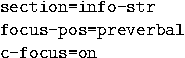
\includegraphics{pdf/choices-frr.pdf} \\
b. & {\small Yiddish} \\
   & 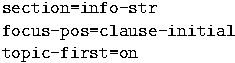
\includegraphics{pdf/choices-ydd.pdf} \\
\end{tabular}
\newpage 
\begin{tabular}{lll}
c. & {\small Miyako} \\
   & 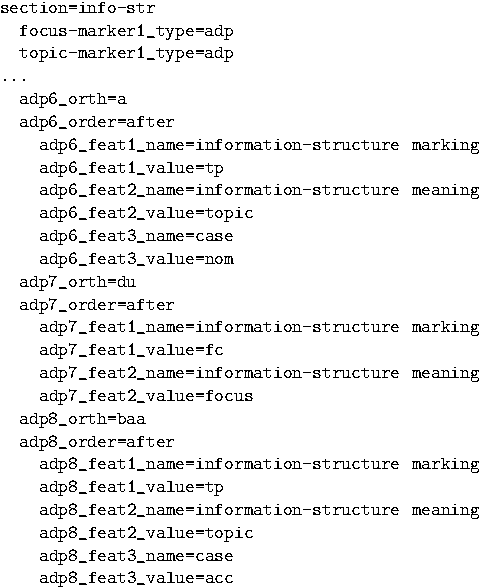
\includegraphics{pdf/choices-mvi.pdf} \\
d. & {\small Lakota} \\
   & 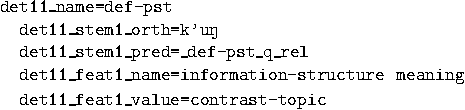
\includegraphics{pdf/choices-lkt.pdf} \\
\end{tabular}}}





\subsection{Testsuites}
\label{12:ssec:lc-testsuites}


The numbers of sentences in each testsuite for the four languages are
shown in Table~\ref{tbl:lc:testsites}. Note that testsuites consist of
both grammatical sentences and ungrammatical sentences.  Each
testsuite also includes test items that represent how information
structure is configured for the language.\is{testsuites}\il{Frisian}\il{Yiddish}\il{Miyako}\il{Yiddish}


\begin{table}[!t]
\small
\centering
\caption{\# of test items}
\label{tbl:lc:testsites}
\begin{tabular}{lrrr}
\lsptoprule
\textbf{language} & \textbf{\# of total items} & \textbf{\# of grammatical items}  & \textbf{\# of information-structure}\\
& & & \textbf{related items} \\ \hline
\midrule
Frisian & 164 & 109  & 6\\
Yiddish  & 228 & 150 & 6\\
Miyako & 102 & 71 & 6\\
Lakota & 168 & 100 & 2 \\
\lspbottomrule 
\end{tabular}
\end{table}




\subsection{Comparison}
\label{12:ssec:lc-comp}


The data set of Language CoLLAGE includes the final grammar and the
\texttt{choices} file, in addition to the testsuite. Using the
\texttt{choices} file, I created two different versions. One was
customized by the previous library, and the other was customized by
the new library. These two versions of grammars are represented as
`old' and `new' respectively hereafter.  I ran these two grammars plus
the final grammar (`final') provided by each developer to see the
coverage and the number of parse trees.  Using the \isi{\lkb} and
\isi{\itsdb}, I parsed all test items in the testsuites for each
language, and then examined how many sentences were covered by each
grammar (i.e.\ coverage) and how many readings were produced
(i.e.\ number of parse trees).


First, coverage of these three types of grammars are compared.  The
grammars created only using the \texttt{choices} file include the main
linguistic modules that can be fully created on the \lingo
\isi{Grammar Matrix} customization system, while the final grammars
(`final') contain more elaborated types and rules that developers
manually edited. Accordingly, the final grammars always yield better
coverage than the other two versions of each grammar. Regarding `old',
and `new', ideally, the coverage between the grammars created by the
old library and those created by the new library should be the same.
That is to say, the distinction between handling grammatical sentences
and ungrammatical sentences should not have changed.  The coverage
that each grammar produced were calculated as shown in Table 12.3.  As
indicated in the third and fourth columns of Table 12.3, there was no
difference in coverage between the two versions of the grammars.


Second, the number of parse trees (i.e.\ readings) may or may not have
changed. This is because I elaborated phrase structure rules that
place constraints on syntactic positioning of marking information
structure.\is{syntactic positioning} In particular, one of the main
components that I refined in the newer version is a routine that deals
with narrow foci in V2 languages.\is{V2 languages} In fact, the old version had a
vulnerability in constraining narrow foci in V2 languages, and
syntactic composition did not work well.\is{narrow focus}  As shown in the third and
fourth column of Table 12.4, the numbers of parse trees produced by
the grammars in \ili{Miyako} and \ili{Lakota} are the same, while
those in V2 languages increase in the new versions. I manually checked
whether the newly produced parse trees were properly constructed and
their semantic representations were correct.  That implies that the
newer version performs better.\il{Frisian}\il{Yiddish}\il{Miyako}\il{Yiddish}



\begin{table}[!t]
\small
\centering
\begin{tabular}{lrrr}
\multicolumn{4}{c}{Table 12.3: Coverage (\%)}\\
\lsptoprule
\textbf{language} & \textbf{final} & \textbf{old}  & \textbf{new} \\ \hline
\midrule
Frisian  & 70.6 &  45.0 &  45.0 \\
Yiddish  & 60.0 &  32.0 &  32.0 \\
Miyako  & 77.5 &  38.0 &  38.0 \\
Lakota  & 91.0 &  60.0 &  60.0 \\
\lspbottomrule
\end{tabular}
\mbox{ }  \mbox{ } \mbox{ }  \mbox{ } \mbox{ }  
\begin{tabular}{lrrr}
\multicolumn{4}{c}{Table 12.4: \# of readings}\\
\lsptoprule
\textbf{language} & \textbf{final} & \textbf{old}  & \textbf{new} \\ \hline
\midrule
Frisian  & 178 &  195 &  209 \\
Yiddish  & 118 &  97 &  98 \\
Miyako  & 80 &  34 &  34 \\
Lakota  & 103 & 62 &  62 \\
\lspbottomrule
\end{tabular}
\end{table}



\subsection{Information structure in the four languages}
\label{12:ssec:lc-info}


Finally, I checked out how information-structure related test items,
whose numbers are given in the last column of
Table~\ref{tbl:lc:testsites}, were parsed and represented in the ICONS
list.  I found that the customized grammars had complete
coverage over these items and returned correct analyses.



\ili{Frisian}, a V2 language,\is{V2 languages} is specified as placing focused constituents
in the preverbal position irrespective of \isi{contrastiveness}.\is{\textit{info-str}}  As
discussed before in Section \ref{11:ssec:ph}, this language includes
\tdl{head-nf-comp-phrase-super}, \tdl{nf-comp-head-phrase}, and
\tdl{narrow-focused-phrase}.\is{narrow focus} The value of \tdl{info-str} that
\isi{preverbal} foci have is \tdl{focus} which can be used for both
\tdl{semantic-focus} and \tdl{contrast-focus}.\is{semantic focus}\is{contrastive focus}

Yiddish employs focus/\isi{topic}-fronting. The grammar for Yiddish also
includes \tdl{head-nf-comp-phrase-super}, \tdl{nf-comp-head-phrase},
and \tdl{narrow-focused-phrase} like \ili{Frisian}, and the value of
\tdl{info-str} that fronted constituents involve is constrained as
\tdl{focus-or-topic}.


Three adpositions that mark information structure in \ili{Miyako} were
also inspected.\is{adposition}  For example, the nominative \isi{topic} marker \textit{a}
in Miyako is customized as follows.


\myexe{\enumsentence{\label{tdl:mvi}
\evnup{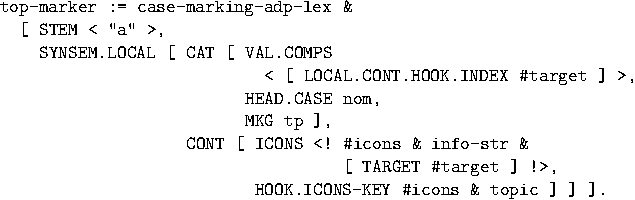
\includegraphics{pdf/tdl-mvi.pdf}}}}


\noindent The adpositions introduce an \tdl{info-str} element into
ICONS, and the value is successfully copied up the trees.\is{\textit{info-str}}  


The \isi{topic}-marking determiner \textit{\textipa{k'u\ng}} in \ili{Lakota}
is an instance of \tdl{def-pst-determiner-lex} in the grammar, and the
type is described as follows.

\myexe{\enumsentence{\label{tdl:lkt}
\evnup{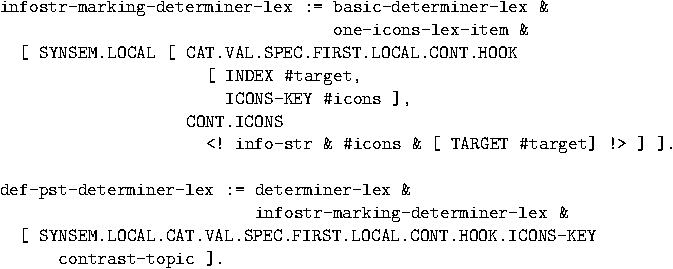
\includegraphics{pdf/tdl-lkt.pdf}}}}

\noindent The \tdl{infostr-marking-determiner-lex} type includes an
element in CONT{$\mid$}ICONS (i.e.\ \tdl{one-icons-lex-item}),
and \tdl{def-pst-determiner-lex}
constrains the value as \tdl{contrast-topic}.  This value comes from
the user's choice given in (\ref{tdl:ho:choices}d).


\subsection{Summary}
\label{11:ssec:lc:sum}

This section substantiates whether my newer version of the information
structure library works well using four grammars and \texttt{choices}
provided in \isi{Language CoLLAGE} (\ili{Frisian}, \ili{Lakota},
\ili{Miyako}, and \ili{Yiddish}). I customized four old versions of
grammars as well as four new versions of grammars using the
\texttt{choices} files. Exploiting the \isi{testsuites} also included
in Language CoLLAGE, I ran the grammars to see if there was no change
in coverage, and how many parse trees were produced. Notably, I
recognized that the newer version yielded better performance in
manipulating information structure in V2 languages (Frisian and
Yiddish).\is{V2 languages}  Additionally, I verified that information structure values
were properly constrained and the values were incrementally augmented
in the \isi{ICONS} list.  In summary, I confirmed that the newer
version correctly operated at least with these four languages.




\section{Live-site}
\label{11:ssec:livesite}

All the components of the information structure library (e.g.\ 
web-based questionnaire, the Matrix-core in \isi{TDL}, and the
Python code for validation and customization) were successfully
implemented in the \lingo \isi{Grammar Matrix} system. The library for
information structure was added in the live site of the customization
system, whose url is presented below. 


\myexe{\enumsentence{\label{def:url:customize}
\myurl{http://www.delph-in.net/matrix/customize}}}


\noindent Thereby, the functionality of the information structure
library is now available for all users of the Grammar Matrix
customization system.



\section{Download}
\label{11:ssec:download}


The source code is downloadable in the subversion repository of the
\lingo Grammar Matrix system (\ref{def:url}a). The specific version
that the present study describes is separately provided, and can be
obtained from (\ref{def:url}b). This version is also independently
served in another web page, whose url is (\ref{def:url}c).


\myexe{\eenumsentence{\label{def:url}
\item \myurl{svn://lemur.ling.washington.edu/shared/matrix/trunk}
\item \myurl{svn://lemur.ling.washington.edu/shared/matrix/branches/sanghoun}
\item \myurl{http://depts.washington.edu/uwcl/sanghoun/matrix.cgi}}}




